%%%%%%%%%%%%%%%%%%%%%%%%%%%%%%%%%%%%%%%%%
% Journal Article
% LaTeX Template
% Version 1.4 (15/5/16)
%
% This template has been downloaded from:
% http://www.LaTeXTemplates.com
%
% Original author:
% Frits Wenneker (http://www.howtotex.com) with extensive modifications by
% Vel (vel@LaTeXTemplates.com)
%
% License:
% CC BY-NC-SA 3.0 (http://creativecommons.org/licenses/by-nc-sa/3.0/)
%
%%%%%%%%%%%%%%%%%%%%%%%%%%%%%%%%%%%%%%%%%

%----------------------------------------------------------------------------------------
%	PACKAGES AND OTHER DOCUMENT CONFIGURATIONS
%----------------------------------------------------------------------------------------

\documentclass[twoside,twocolumn]{article}

\usepackage{blindtext} % Package to generate dummy text throughout this template

\usepackage[sc]{mathpazo} % Use the Palatino font
\usepackage[T1]{fontenc} % Use 8-bit encoding that has 256 glyphs
\linespread{1.05} % Line spacing - Palatino needs more space between lines
\usepackage{microtype} % Slightly tweak font spacing for aesthetics

\usepackage[english]{babel} % Language hyphenation and typographical rules
\usepackage{graphicx}

\usepackage[hmarginratio=1:1,top=32mm,columnsep=20pt]{geometry} % Document margins
\usepackage[hang, small,labelfont=bf,up,textfont=it,up]{caption} % Custom captions under/above floats in tables or figures
\usepackage{booktabs} % Horizontal rules in tables

\usepackage{lettrine} % The lettrine is the first enlarged letter at the beginning of the text
\usepackage{algorithm}
\usepackage[noend]{algpseudocode}
\usepackage{amsmath}

\usepackage{enumitem} % Customized lists
\setlist[itemize]{noitemsep} % Make itemize lists more compact

\usepackage{abstract} % Allows abstract customization
\renewcommand{\abstractnamefont}{\normalfont\bfseries} % Set the "Abstract" text to bold
\renewcommand{\abstracttextfont}{\normalfont\small\itshape} % Set the abstract itself to small italic text

\usepackage{titlesec} % Allows customization of titles
\renewcommand\thesection{\Roman{section}} % Roman numerals for the sections
\renewcommand\thesubsection{\roman{subsection}} % roman numerals for subsections
\titleformat{\section}[block]{\large\scshape\centering}{\thesection.}{1em}{} % Change the look of the section titles
\titleformat{\subsection}[block]{\large}{\thesubsection.}{1em}{} % Change the look of the section titles

\usepackage{fancyhdr} % Headers and footers
\pagestyle{fancy} % All pages have headers and footers
\fancyhead{} % Blank out the default header
\fancyfoot{} % Blank out the default footer
\fancyhead[C]{Running title $\bullet$ May 2016 $\bullet$ Vol. XXI, No. 1} % Custom header text
\fancyfoot[RO,LE]{\thepage} % Custom footer text

\usepackage{titling} % Customizing the title section

\usepackage{hyperref} % For hyperlinks in the PDF

%----------------------------------------------------------------------------------------
%	TITLE SECTION
%----------------------------------------------------------------------------------------

\setlength{\droptitle}{-4\baselineskip} % Move the title up

\pretitle{\begin{center}\Huge\bfseries} % Article title formatting
\posttitle{\end{center}} % Article title closing formatting
\title{Baysian Optimization in MPC} % Article title
\author{%
\textsc{Frederic Dlugi}\\[1ex] % Your name
\normalsize Universität zu Lübeck \\ % Your institution
\normalsize \href{mailto:frederic.dlugi@student.uni-luebeck.de}{frederic.dlugi@student.uni-luebeck.de} % Your email address
%\and % Uncomment if 2 authors are required, duplicate these 4 lines if more
%\textsc{Jane Smith}\thanks{Corresponding author} \\[1ex] % Second author's name
%\normalsize University of Utah \\ % Second author's institution
%\normalsize \href{mailto:jane@smith.com}{jane@smith.com} % Second author's email address
}
\date{\today} % Leave empty to omit a date
\renewcommand{\maketitlehookd}{%
\begin{abstract}
\noindent \blindtext % Dummy abstract text - replace \blindtext with your abstract text
\end{abstract}
}

%----------------------------------------------------------------------------------------

\begin{document}

% Print the title
\maketitle

%----------------------------------------------------------------------------------------
%	ARTICLE CONTENTS
%----------------------------------------------------------------------------------------

\section{Introduction}

\lettrine[nindent=0em,lines=3]{W} e start by introducing bayesian optimization and MPC on a high level.
This is done to let you know what I understand when talking about these algorithms.

\subsection{What is Bayesian Optimization?}
Bayesian optimization is a strategy for global optimization of backbox functions.
It therefore does not require the computation of gradients, but works best on continuous functions.
It is best suited for optimizing functions, where each evaluation takes a long time.
The number of input dimensions for bayesian optimization is typically less then $20$.\cite{frazier2018tutorial}

\begin{algorithm}
    \caption{Bayesian Optimization}
    \begin{algorithmic}
        \State $\text{f} \gets \text{black box function}$
        \State $\text{initPos} \gets \text{initial positions}$
        \State $\text{evaluations} \gets \text{f(initPos)}$
        \State $\alpha \gets \text{calcAquisitionFunction(evaluations)}$
        \For{$i= 1 \to N$}
            \State $\text{nextPos} \gets \text{argmax(}\alpha\text{)}$
            \State $\text{evaluations}.append(\text{f(nextPos)})$
            \State $\alpha \gets \text{calcAquisitionFunction(evaluations)}$
        \EndFor
        \State $result \gets \text{max(evaluations)}$
    \end{algorithmic}
\end{algorithm}

\subsection{What is MPC?}
MPC is an acronym for model predicive control.
It replaces classical control algorithms that usually work in an offline manner with an optimizer,
that solves the optimal control problem for a receding horizon (Figure \ref{fig:mpc}).
Each action taken is the first action of the optimal control plan.
The plan gets updated continuously (Figure \ref{fig:mpc_plan}).

\begin{figure}[h]
    \caption{Blockdiagram of MPC algorithm}
    \centering
    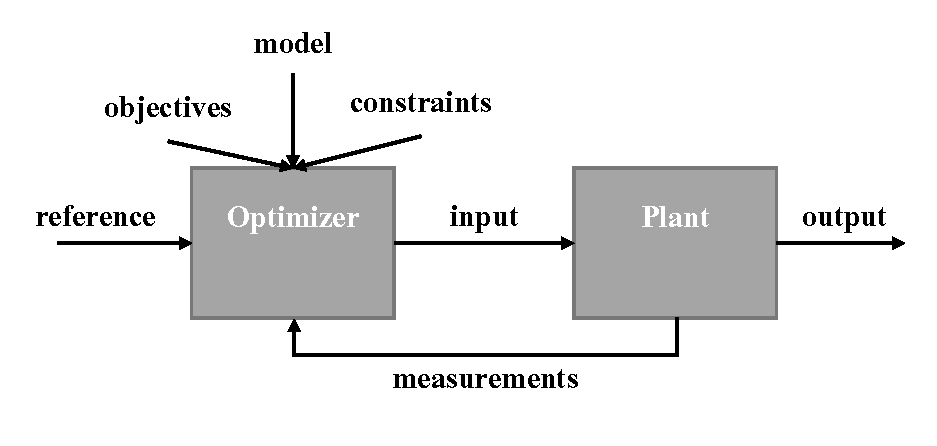
\includegraphics[width=0.45\textwidth]{fig_mpc.pdf}
    \label{fig:mpc}
\end{figure}

\begin{figure}[h]
    \caption{Plan horizon of MPC algorithm}
    \centering
    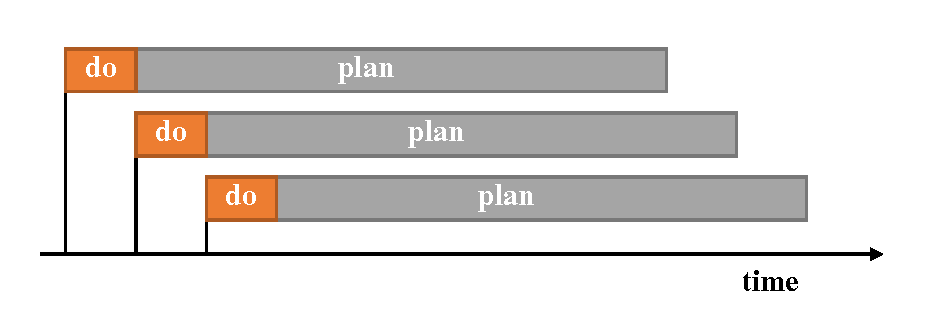
\includegraphics[width=0.45\textwidth]{fig_mpc_plan.pdf}
    \label{fig:mpc_plan}
\end{figure}

%------------------------------------------------

\section{Methods}

Maecenas sed ultricies felis. Sed imperdiet dictum arcu a egestas.
\begin{itemize}
\item Donec dolor arcu, rutrum id molestie in, viverra sed diam
\item Curabitur feugiat
\item turpis sed auctor facilisis
\item arcu eros accumsan lorem, at posuere mi diam sit amet tortor
\item Fusce fermentum, mi sit amet euismod rutrum
\item sem lorem molestie diam, iaculis aliquet sapien tortor non nisi
\item Pellentesque bibendum pretium aliquet
\end{itemize}
\blindtext % Dummy text

Text requiring further explanation\footnote{Example footnote}.

%------------------------------------------------

\section{Results}

\begin{table}
\caption{Example table}
\centering
\begin{tabular}{llr}
\toprule
\multicolumn{2}{c}{Name} \\
\cmidrule(r){1-2}
First name & Last Name & Grade \\
\midrule
John & Doe & $7.5$ \\
Richard & Miles & $2$ \\
\bottomrule
\end{tabular}
\end{table}

\blindtext % Dummy text

\begin{equation}
\label{eq:emc}
e = mc^2
\end{equation}

\blindtext % Dummy text

%------------------------------------------------

\section{Discussion}

\subsection{Subsection One}

A statement requiring citation \cite{sorourifar2021data}.
\blindtext % Dummy text

\subsection{Subsection Two}

\blindtext % Dummy text

%----------------------------------------------------------------------------------------
%	REFERENCE LIST
%----------------------------------------------------------------------------------------
\bibliographystyle{plain}
\bibliography{refs.bib}
%----------------------------------------------------------------------------------------

\end{document}
